\makeatletter                                                   
\def\input@path{{../}}                                          
\makeatother                                                    
\documentclass[../main.tex]{subfiles}                           
\begin{document}                                                
\chapter{Solution Methods}
\label{ch:methods}

This chapter will go over the most common solution methods in metaheuristics and will be divided up in three parts.
The first part, \cref{sec:requirements} will cover metaheuristics and requirements of a good solution method.
The next \cref{sec:intens} will present approaches that help intensify the search. 
The final part \cref{sec:divers} will focus on approaches that helps a model to diversify the search for solutions. The chapter will lead us to the solution method we have chosen which is presented in detail in \cref{ch:appr}.

\section{Solution method requirements}
\label{sec:requirements}
A metaheuristic is a high-level problem-independent algorithmic framework that provides a set of guidelines or strategies to develop heuristic optimization algorithms \cite{sorensen13}. 
A metaheuristic is therefore by definition a very open way of approaching a problem and many different approaches have been developed in the last few decades.
The most noteable metaheuristics include (adaptive) large neighbourhood search, tabu search, simmulated anealing, genetic algorithm, variable neighbourhood search and ant colonization, among many more. 
The term meta-heuristic was first used by \cite{glover86} when he coined it, aswell as tabu search which he combined with artificial intelligence strategies to build a framework for integer programming. \par

For a metaheuristic algorithm to be efficient it has to be able to generate new solutions that are likely to improve on previous/existing solutions.
At the same time it has to be able to cover the most important parts of the solution space where the global optimum may be found as well as being able to escape a local optimum.
In other words a good metaheuristic approach requires a good balance between two important principles \textit{intensification} and \textit{diversification}. 
A good balance between these principles will help ensure a near global optimal solution.
In the following sections we will go more into details on these two principles.

\begin{figure}
    \centering
    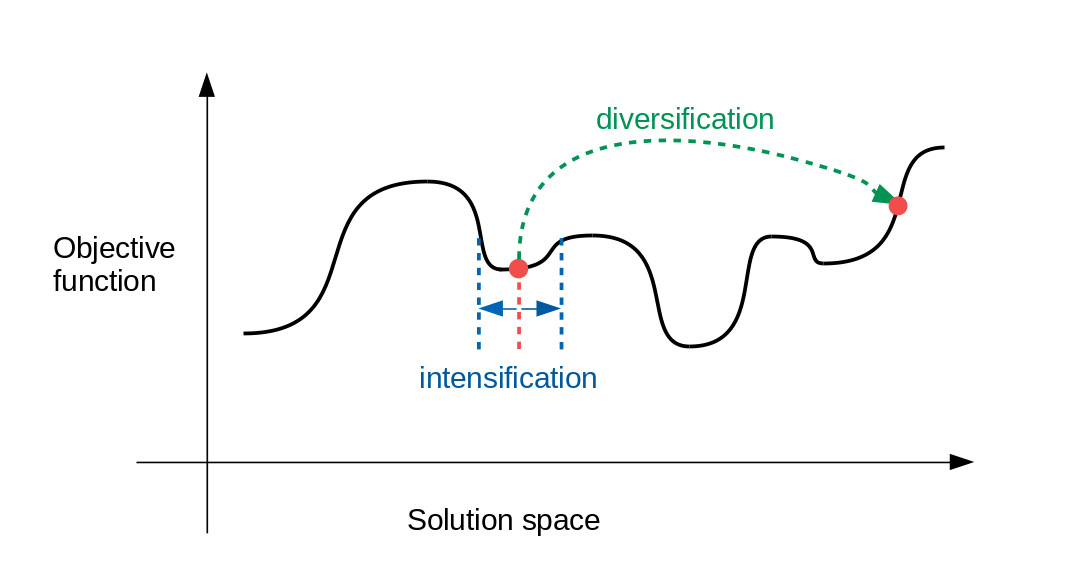
\includegraphics[width=0.8\textwidth]{diver_intensification}
    \caption{The figure illustrates how intensification, in blue, and diversification, in green, works while exploring a solutions space.}
    \label{fig:sification}
\end{figure}

\section{Intensification}
\label{sec:intens}
By intensification we refer to a metaheuristics ability to focus the search on a local region with a good solution in it. 
Too much intensification will lead the algorithm to be trapped in a local optima and will make it nearly impossible to find a global optimal solution. 
In \cref{fig:sification} we show how intensification might work on a given solution space. \par

Local search heuristics like the ones implemented by \cite{nanry00} and \cite{li03} are build using intensification heuristics that perform smaller moves such as moving an order from one vehicle to another, or swapping two orders with eachother. 
We implemented two similar heuristics in \cref{sec:swap} and \cref{sec:exch} which are performing small efficient intensification moves. \par
\cite{lin65} implemented a 2-opt heuristic for travelling salesman problem. The 2-opt heuristic is a very intensification operator as it focuses on one vehicles routes neighbourhood through several iterations and ends up returning the local optimum for that vehicle route. We have implemented a version of the 2-opt heuristic in \cref{sec:2opt}.

\section{Diversification}
\label{sec:divers}
Diversification refers to a metaheuristics ability to explore the solution space on a global scale by generating diverse solutions. 
Too much diversification will lead to a random search that will make it hard for the algorithm to converge to a local optima, and it will slow down the overall search performance. 
\Cref{fig:sification} illustrates how diversification is working on a solution space. \par

\cite{cordeau01} diversified by relaxing constraints and thereby allowing the search to visit infeasible solutions. In \cref{sec:wild} we have implemented a diversifying escape algorithm that successfully allows our algotihm to escape one part of a solution space and move to new unexplored areas, as we show in \cref{sec:evalW} \par
Large neighbourhood search (\textit{LNS}) was introduced by \cite{shaw97} and this metaheuristic diversifies by removing and reinserting a certain amount of orders $q$ in each iteration. 
Our implementation will be based on a similar type of framework as LNS.

\begin{algorithm}
    \caption{Large neighbourhood search}\label{alg:lns}
    \begin{algorithmic}[1]
        \Function{LNS}{solution s}
        \State solution $s_{best} = s$
        \Repeat
            \State $s' = s$
            \State select number of orders to remove $q$
            \State remove $q$ orders from $s'$
            \State insert removed orders in $s'$
            \If {$f(s') < f(s_{best})$}
                \State $s_{best}=s'$
            \EndIf
            \If {$accept(s', s)$}
                \State $s = s'$
            \EndIf
        \Until {stop condition met}
        \State
        \Return $s_{best}$
        \EndFunction
    \end{algorithmic}
\end{algorithm}

\Cref{alg:lns} shows a pseudocode of the LNS algorithm which is given a starting solution $s$. 
First the algorithm updates the best solution $s_{best}$ as the given $s$.
It then goes into a loop which runs until a stop condition is met.
Here it selects a number of orders $q$ to remove from the current solution $s'$.
The algorithm then inserts the removed orders back into the current solution $s'$. The removal and insertion procedures are selected separately. The amount of orders $q$ is influencing if the algorithm will perform a very diversified action or a very intensified operation.
In our model we have chosen to let the  heuristics choose how many orders to operate on between a certain interval $[1,..m]$ where $m$ is $10\%$ of the total amount of orders. 
We believe this will let our heuristics have a good balance between intensification and diversification. \par

After removing and inserting orders, the $s_{best}$ is updated if the new solution results in a better objective value. 
Then the solution $s$ is updated if the solution is accepted. 
\cite{shaw97} chose to accept solutions that are better than the current one. We will implement a different acceptance criteria which we will present below. \par

\cite{ropke06} implemented a version of the LNS called Adaptive large neighbourhood search. He changed the LNS to adapt itsself by keeping track of the performance of each heuristic. 
In \cref{sec:weight} we have used similar adaptive weights to allow our model to automatically keep a good balance between diversification and intensification. \par

The tabu search implemented by \cite{glover86} uses a memory, or a tabu list, which remembers parts of the search which are then being cut off, or tabu'ed.
This type of behaivior helps the algorithm to diversify and avoid searching in a cycle by performing the same type of move. 
We have chosen to remember which solutions we have visited and not rewarding this type of behaivior in our adaptive weights. \par

\cite{kirkpatrick83} implemented a simmulated anealing algorithm applied to the travelling salesmen problem. Simmulated anealing helps diversify a search by sometimes accepting worse solutions based on a temperature $T$. 
The temperature $T$ is on a cooling down schedule and the longer the search goes on the lower the chances of acceptance becomes. 
In \cref{sec:accept} we have used a similar acceptance criteria in our model.

The proposed solution method, which we call \textit{the fourth party logistics optimizer}, is trying to balance the intensification and diversification to solve the 4PL problem. The complete model is explained in detail in the next chapter.
\biblio
\end{document}  
